\usepackage[utf8]{inputenc}
\usepackage[T1]{fontenc}
\usepackage[ngerman]{babel}
\usepackage{avant}
\mode<article>{\usepackage{tgschola}}

\usepackage{listings}

\usepackage{tikz}
\usetikzlibrary{intersections}
\usetikzlibrary{arrows,decorations.pathmorphing,backgrounds,positioning,fit}


\mode<presentation>{\beamertemplatenavigationsymbolsempty}

\usetheme{Laser}

\mode<article>{
\newenvironment{niitemize}{
\begin{itemize}}{\end{itemize}}
}

\makeatletter
\mode<presentation>{
\newenvironment{niitemize}{
  \ifnum\@itemdepth >2\relax\@toodeep\else
      \advance\@itemdepth\@ne%
      \beamer@computepref\@itemdepth%
      \usebeamerfont{itemize/enumerate \beameritemnestingprefix body}%
      \usebeamercolor[fg]{itemize/enumerate \beameritemnestingprefix body}%
      \usebeamertemplate{itemize/enumerate \beameritemnestingprefix body begin}%
      \begin{list}
        {
            \usebeamertemplate{itemize \beameritemnestingprefix item}
        }
        { \leftmargin=1.2em \itemindent=0em
            \def\makelabel##1{%
              {%
                  \hss\llap{{%
                    \usebeamerfont*{itemize \beameritemnestingprefix item}%
                        \usebeamercolor[fg]{itemize \beameritemnestingprefix item}##1}}%
              }%
            }%
        }
  \fi
}
{
  \end{list}
  \usebeamertemplate{itemize/enumerate \beameritemnestingprefix body end}%
}
}
\makeatother

\setbeamercolor{normal text}{fg=black,bg=black!2}

\lstset{
columns=fullflexible,
basicstyle=\ttfamily,
}


\newcommand{\LA}{\ensuremath{\Leftarrow}}
\newcommand{\la}{\ensuremath{\leftarrow}}
\newcommand{\RA}{\ensuremath{\Rightarrow}}
\newcommand{\ra}{\ensuremath{\rightarrow}}
\newcommand{\lra}{\ensuremath{\leftrightarrow}}
\newcommand{\On}{\ensuremath{O(n)}\xspace}
\newcommand{\Ologn}{\ensuremath{O(\log n)}\xspace}
\newcommand{\Oone}{\ensuremath{O(1)}\xspace}

\title{Presslufthammer}
\subtitle{Final Presentation}
\date{WiSe 2011/12}
\author{Aljoscha Krettek \and Fabian Eichhorn}
\institute
{
  \inst{}
  DIMA\\
  Technische Universität Berlin
}
\subject{Textmining}

\begin{document}

\begin{frame}[t,plain]
\titlepage
\end{frame}

\begin{frame}[t,plain]{Agenda}
\tableofcontents
\end{frame}

\section{Project Overview}

\begin{frame}<presentation>{Project Overview}
\begin{niitemize}
 \item Open source implementation prototype of Google BigQuery, based on Dremel
   paper\footnote{http://research.google.com/pubs/pub36632.html}
 \item Handling of mostly aggregation queries on very large data
 \item Data stored in novel columnar format on cluster of machines
 \item Hierarchy of compute nodes for interactive query performance
 \item SQL-like query language
\end{niitemize}
\end{frame}

\section{Storage}

\begin{frame}<presentation>{Hierarchical vs. Columnar}
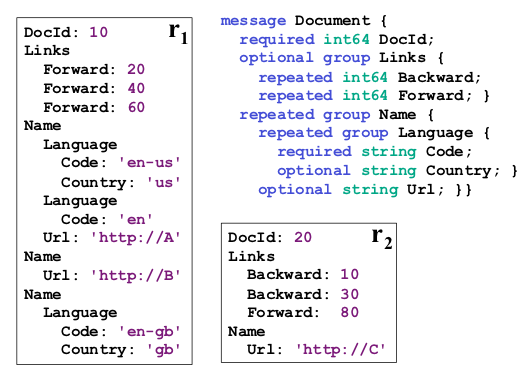
\includegraphics[width=.49\textwidth]{gfx/hierarchical-schema}
\hfill
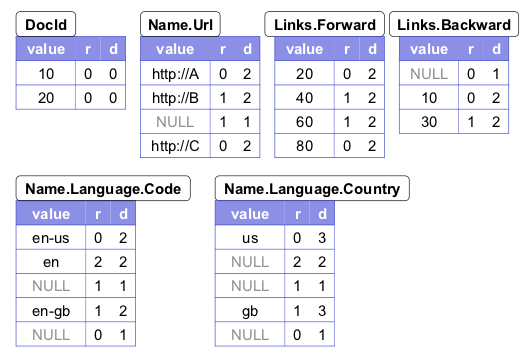
\includegraphics[width=.5\textwidth]{gfx/columnar}

\begin{niitemize}
 \item Repetition/Definition levels represent record structure
 \item \texttt{FieldStriper} stripes records to columns
 \item \texttt{AssemblyFSM} assembles records from columns
\end{niitemize}
\end{frame}

\begin{frame}<presentation>{Record Striping}
\begin{niitemize}
 \item Recursively stripe record from a \texttt{RecordStore} using a
  \texttt{RecordDecoder} and tree of \texttt{FieldWriter}S
 \item Implementation of \texttt{RecordStore} and \texttt{RecordDecoder} only
  for JSON for now
 \item Data written to a \texttt{Tablet} using a \texttt{ColumnWriter}
 \item Implementation of \texttt{ColumnWriter} and \texttt{Tablet} for on-disk
  storage and in-memory so far
\end{niitemize}
\end{frame}

\begin{frame}<presentation>{Record Assembly}
\begin{niitemize}
 \item Assemble records to a \texttt{RecordStore} using a
  \texttt{RecordEncoder} using \texttt{AssemblyFSM}
 \item Read columnar data from \texttt{Tablet} using a \texttt{ColumnReader}
\end{niitemize}

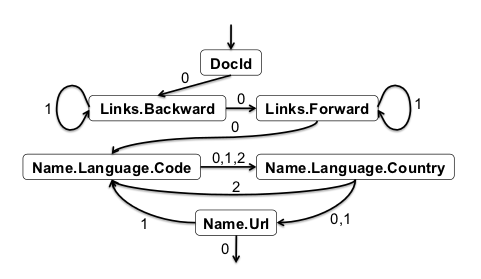
\includegraphics[width=.49\textwidth]{gfx/full-assemblyfsm}
\hfill
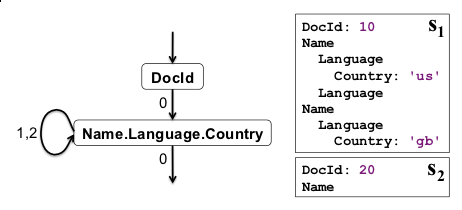
\includegraphics[width=.49\textwidth]{gfx/partial-assemblyfsm}
\end{frame}

\begin{frame}<presentation>{Storage Layer}
\begin{niitemize}
 \item For now we use local file system to store columnar data
 \item System is general enough to allow other storage backends
 \item Could implement proprietary storage layer:
   \begin{niitemize}
     \item Need to handle fault tolearnce, replication ...
     \item Better optimized for task
   \end{niitemize}
 \item Use HDFS for storage layer:
   \begin{niitemize}
     \item Has most stuff out-of-box
     \item Not as efficient
   \end{niitemize}
\end{niitemize}
\end{frame}

\begin{frame}<presentation>{Issues}
\begin{niitemize}
 \item Data format difficult to understand, sometimes descriptions
  in paper inconsistent
 \item ``Algorithms'' in paper for striping, assembly and query processing are only
  rough sketch, still required lot of
  thinking/debugging
\end{niitemize}
\end{frame}


\section{Query Execution}


\begin{frame}<presentation>[fragile]{Supported Queries}
\begin{niitemize}
  \item We support select-project-aggregate queries with where clauses in pseudo-SQL language
  \item Renaming is supported
  \item COUNT and SUM as aggregation functions
  \item Only != and == operators in expressions, combining expressions only with OR
  \item Uses columnar data throughout, only last result as
    records (hierarchical) to client
  \item Columnar data read from source tablet into target tablet, ignoring
    columns that are projected out
\end{niitemize}
\end{frame}

\begin{frame}<presentation>[fragile]{Query Execution}
\begin{niitemize}
 \item Query parser using ANTLR
 \item Semantical analysis (very basic for now)
 \item Query rewriting (Schema rewriting):
   \begin{niitemize}
     \item \verb#SELECT COUNT(bla) FROM Foo# \ra{} \verb#SELECT COUNT(bla) FROM Foo:x# and
       \verb#SELECT SUM(bla) FROM Foo#
   \end{niitemize}
 \item Query execution on leafs
 \item Grouping is hash based, so system blows up with too many groups\footnote{Also the case with Google BigQuery}
\end{niitemize}
\end{frame}

\begin{frame}<presentation>{Issues}
\begin{niitemize}
 \item Query processing only sketched in paper, only basic
  select-project-aggregate
 \item Is rather slow because for every emitted value the where expressions
  are evaluated
 \item Would greatly benefit from JIT
\end{niitemize}
\end{frame}

\section{Network}
\begin{frame}<presentation>{Network}
  Dremel architecture consists of four types of nodes
  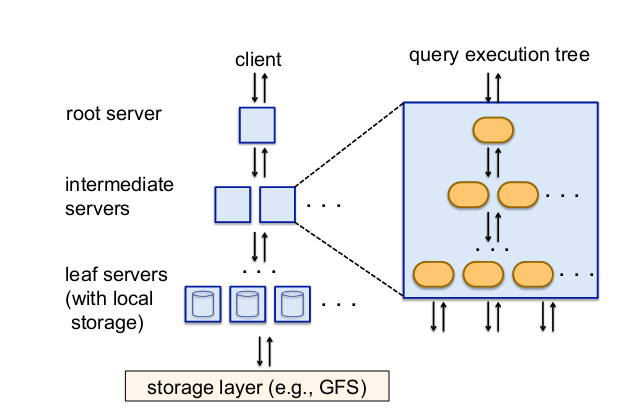
\includegraphics[width=.55\textwidth]{gfx/net-arch}
  \begin{niitemize}
    \item Coordinator
    \item Inner
    \item Leaf and
    \item Client Nodes
  \end{niitemize}
\end{frame}

\begin{frame}<presentation>{Coordinator and Inner Nodes}
  Coordinator Node
  \begin{niitemize}
    \item Central entry point
    \item Accepts Queries from Clients
    \item Hands Out Jobs to Leafs
  \end{niitemize}
  Inner Nodes
  \begin{niitemize}
    \item Not Implemented
    \item Build an intermediate layer
    \item Take care of splitting/aggregating queries
  \end{niitemize}
\end{frame}

\begin{frame}<presentation>{Leaf and Client Nodes}
  Leaf Node
  \begin{niitemize}
    \item Connection between Network and Storage
    \item Data fetching / Storage Access
    \item Per Tablet Query processing
  \end{niitemize}
  Client Node
  \begin{niitemize}
    \item Provides the UI
    \item Attaches to a Coordinator
    \item CLI or Jetty based
  \end{niitemize}
\end{frame}

\begin{frame}<presentation>{Slave Nodes}
  Slave Node
  \begin{niitemize}
    \item Leaf and Inner functionality combined
    % \item Data fetching / Storage Access
    \item Arrange themselves in an n-ary tree
    \item Take care of splitting/aggregating queries
    % \item Per Tablet Query processing
  \end{niitemize}
\end{frame}

\begin{frame}<presentation>{Issues}
  \begin{niitemize}
   \item Coordination of Nodes: Intermediate Layer
   \item Proper Serialization of Meta-Data for Transfer
   \item Fault tolerance / Reconfigurability
  \end{niitemize}
\end{frame}



\section{Conclusions and Further Work}
\begin{frame}<presentation>{Further Work}
\begin{niitemize}
  \item Implementation of a purely intermediate layer
  \item Implementation of a distributed storage layer
  \item Implementation of a richer graphical user interface
  \item Improving fault tolerance
  \item Testing and Evaluation of distributed execution
  \item Performance evaluation at scale
  \item Proper semantical analysis of queries
  \item Join of several tables
  \item Optimization of queries
  \item Code generation for query execution
\end{niitemize}
\end{frame}

\end{document}
